% A skew Hadamard matrix of order 2120
% Compile with pdflatex (see the repository Makefile).

\documentclass[11pt]{article}
\usepackage[margin=1in]{geometry}
\usepackage[T1]{fontenc}
\usepackage{amsmath,amssymb,amsthm}
\usepackage{tikz}
\usepackage[colorlinks=true,linkcolor=blue,citecolor=blue,urlcolor=blue]{hyperref}
\newtheorem{theorem}{Theorem}
\newtheorem{lemma}[theorem]{Lemma}
\newtheorem{corollary}[theorem]{Corollary}
\theoremstyle{remark}
\newtheorem{remark}[theorem]{Remark}
\newcommand{\F}{\mathbb F}
\newcommand{\one}{\mathbf 1}
\setlength{\emergencystretch}{3em}
\hypersetup{
  pdftitle={A skew Hadamard matrix of order 2120},
  pdfauthor={Jeffery Kline}
}

\title{A skew Hadamard matrix of order 2120}
\author{Jeffery Kline}
\date{Release candidate, November 2026}

\begin{document}
\maketitle

\begin{abstract}
We construct a skew Hadamard matrix of order $2120=2^3\cdot265$. We found no earlier published construction at this order. The Cati--Pasechnik database records $4240=2^4\cdot265$ as the least known skew order with odd part $265$, and the 2025 census of \DJ{}okovi\'c and Seberry lists order $1060$ as undecided. The matrix comes from four sign masks on the field of $529=23^2$ elements whose Fourier energies sum to a constant. Each mask is fixed by eight signs on the projective line over $\F_{23}$. A table of eight integer character sums certifies the construction, and the sums can be checked by hand. A classical bordered array then gives the matrix. On the same field the cyclotomic families of Momihara and Xiang have eight blocks, and their matrix constructions use at most four. A vector form of Turyn's cyclic expansion carries the four masks to every odd power. The same method works with seeds in characteristics $7$ and $263$. It gives skew Hadamard matrices of order $4(p^{2n}+1)$ for $p\in\{7,23,263\}$ and every odd $n\ge1$; the seed at $263$ rests on a machine computation. Four is the least number of blocks possible for an all-skew family on these groups.
\end{abstract}

\section{Introduction}
A Hadamard matrix $H$ of order $N$ is \emph{skew} if $H+H^T=2I$. Skew Hadamard matrices are conjectured to exist for every $N\equiv0\pmod 4$. Since a skew matrix of order $N$ gives one of order $2N$, the existence question for odd $m$ reduces to the least exponent $t$ such that a skew matrix of order $2^tm$ is known. Cati and Pasechnik tabulate this exponent~\cite[Table~5]{CP}. For $m=265$ they record $t=4$, from order $4240$. \DJ{}okovi\'c and Seberry's census of skew orders $4v$ with odd $v<2500$ lists $v=265$, that is order $1060$, among the undecided cases~\cite{DS}.

\begin{theorem}\label{main}
There is an explicit skew Hadamard matrix of order $2120$. Hence the least exponent for odd part $265$ is at most three.
\end{theorem}

The construction has two steps. First, we find four odd functions $g_1,\dots,g_4\colon\F_{529}\to\{0,\pm1\}$, vanishing only at $0$, whose squared Fourier magnitudes sum to $4\cdot529$ at every nonprincipal character (Section~\ref{sec:seed}). Each $g_i$ scales by the quadratic character of $\F_{23}$ along lines, so it is determined by $24$ signs. These come from one pattern of eight signs, rotated. The energy condition reduces to eight integer sums, listed in Section~\ref{sec:seed}. Second, a bordered Goethals--Seidel-type array turns the four developed blocks into a skew Hadamard matrix of order $4(529+1)$ (Section~\ref{sec:array}).

The method extends in two directions. A vector version of Turyn's cyclic expansion~\cite{Turyn71,Mom} carries any such list of four functions (a \emph{seed}, defined in Section~\ref{sec:array}) on $\F_q$ to $\F_q^{\,n}$ for odd $n$ (Section~\ref{sec:expansion}). Seeds of the same shape exist at $q=7^2$ and $q=263^2$. A parity argument shows that four is the least number of all-skew blocks with this energy condition on these groups (Section~\ref{sec:minimum}).

\paragraph{Relation to known constructions.}
Wallis and Whiteman~\cite{WW} and Momihara and Xiang~\cite{MX} build skew supplementary blocks from cyclotomic classes. On $\F_{529}$, where $529\equiv17\pmod{32}$, their Theorem~1.5 gives an eight-block family, while their matrix corollaries use two or four blocks. The four-block hypothesis of~\cite{MX} needs a base field of order $9\bmod16$, and no subfield of $\F_{23^{2n}}$ has one. Order $4240$ is reached by a product theorem: amicable Hadamard matrices of order $20$ (from $19$) and a Paley skew matrix of order $212$ give a skew matrix of order $20\cdot212$~\cite[Theorem~13]{KS}. The Agayan--Sarukhanyan half-product of the Paley matrices of orders $20$ and $212$ gives an ordinary Hadamard matrix of order $2120$~\cite[Lemma~2.4]{SY}. As written, though, on skew inputs each diagonal entry of its upper-left block is the negative of the corresponding diagonal entry of its lower-right block, so the array has trace zero and is not of the form $I+S$. Paley's construction of skew matrices of order $q+1$, for a prime power $q\equiv3\pmod4$ (Paley I), fails at $2120$ and at $1060$, since $2119=13\cdot163$ and $1059=3\cdot353$. The four masks at $23$ were first found by the author in an unpublished computer search in July 2026. This paper supplies the certificate, the matrix and the extension.

\section{From four masks to a skew Hadamard matrix}\label{sec:array}
Let $V$ be a finite abelian group of odd order $v$. Use unnormalized transforms $\widehat f(u)=\sum_x f(x)u(x)$. A \emph{seed} is a list of odd functions $g_1,\dots,g_4\colon V\to\{0,\pm1\}$ with $g_i(0)=0$ and $g_i(x)=\pm1$ for $x\ne0$, such that
\begin{equation}\label{seed}
\sum_{i=1}^4|\widehat g_i(u)|^2=4v\qquad(u\ne1).
\end{equation}

\begin{lemma}\label{array}
A seed on $V$ gives a skew Hadamard matrix of order $4(v+1)$.
\end{lemma}

\begin{proof}
Put $F_i=\delta_0+g_i$. Since $g_i$ is real and odd, $\widehat g_i$ is purely imaginary, so $|\widehat F_i|^2=1+|\widehat g_i|^2$. At the principal character $\widehat F_i(1)=1$. Fourier inversion of \eqref{seed} gives
\[
\sum_i\sum_xF_i(x)F_i(x+b)=\begin{cases}4v,&b=0,\\-4,&b\ne0.\end{cases}
\]
Let $A_i(x,y)=F_i(y-x)$, let $R$ be the reflection $R(x,y)=[x+y=0]$, and put $D_i=A_iR$ and $T_i=RA_i$. Then $A_i+A_i^T=2I$, the $A_i$ commute with each other and with their transposes, $RA_iR=A_i^T$, and $\sum_iA_iA_i^T=4(v+1)I-4J$. Each $A_i$ has row sums one. Take
\[
 C=\begin{pmatrix}+&+&+&+\\-&+&-&+\\-&+&+&-\\-&-&+&+\end{pmatrix},\quad
 U=\begin{pmatrix}-&-&-&-\\-&-&+&+\\-&+&+&-\\-&+&-&+\end{pmatrix},\quad
 W=\begin{pmatrix}
 A_1&D_2&D_3&D_4\\
 -D_2&A_1&-T_4&T_3\\
 -D_3&T_4&A_1&-T_2\\
 -D_4&-T_3&T_2&A_1
 \end{pmatrix},
\]
and let $H=\begin{pmatrix}C&U\otimes\one^T\\-(U\otimes\one^T)^T&W\end{pmatrix}$, where each sign of $U$ is repeated across a block of $v$ columns. The off-diagonal Gram blocks of $W$ cancel in pairs by the identities above, and each diagonal one is $4(v+1)I-4J$. The lower border adds $4J$. The block row sums of $W$ form the matrix $C$, and the top and mixed Gram blocks follow from $CC^T=UU^T=4I$ and $CU=UC^T$. Thus $HH^T=4(v+1)I$ and $H+H^T=2I$. Figure~\ref{fig:array} shows the layout. This is a bordered variant of the Goethals--Seidel array; compare the bordered arrays in Propositions~1.1 and~1.3 of~\cite{MX}, where only the first block needs to be skew.
\end{proof}

\begin{figure}[t]
\centering
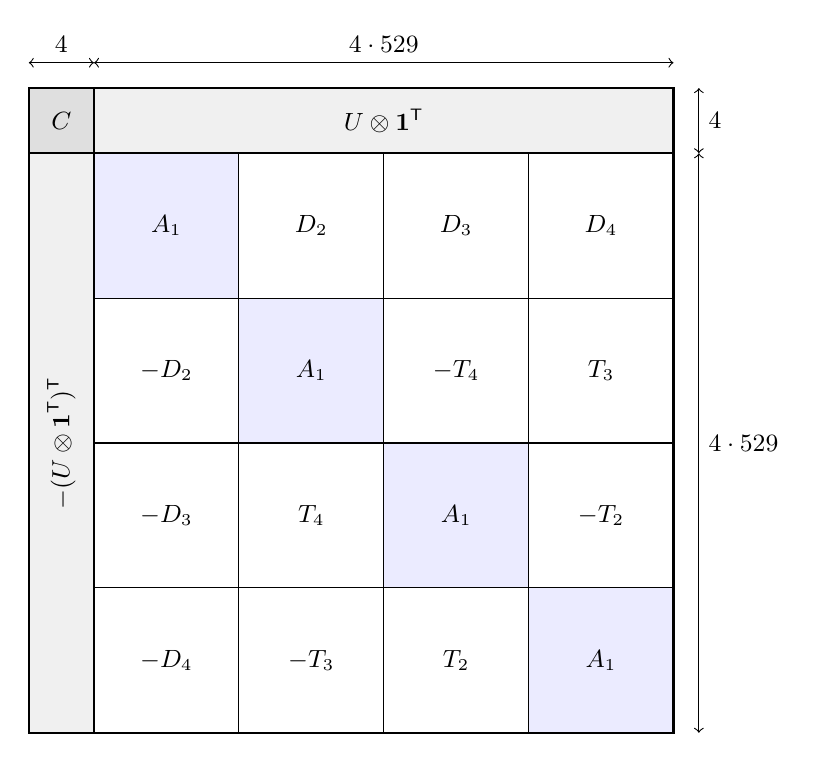
\begin{tikzpicture}[x=0.92cm,y=0.92cm,font=\small]
  % border strips (drawn wider than scale) and core grid
  \def\b{0.9}
  \fill[gray!25] (0,0) rectangle (\b,-\b);
  \fill[gray!12] (\b,0) rectangle (\b+8,-\b);
  \fill[gray!12] (0,-\b) rectangle (\b,-\b-8);
  \foreach \i in {0,...,3} \fill[blue!8] (\b+2*\i,-\b-2*\i) rectangle (\b+2*\i+2,-\b-2*\i-2);
  \draw[thick] (0,0) rectangle (\b+8,-\b-8);
  \draw[thick] (\b,0) -- (\b,-\b-8);
  \draw[thick] (0,-\b) -- (\b+8,-\b);
  \foreach \k in {1,2,3} {
    \draw (\b+2*\k,-\b) -- (\b+2*\k,-\b-8);
    \draw (\b,-\b-2*\k) -- (\b+8,-\b-2*\k);
  }
  \node at (\b/2,-\b/2) {$C$};
  \node at (\b+4,-\b/2) {$U\otimes\mathbf 1^{\mathsf T}$};
  \node[rotate=90] at (\b/2,-\b-4) {$-(U\otimes\mathbf 1^{\mathsf T})^{\mathsf T}$};
  \foreach \r/\row in {0/{A_1,D_2,D_3,D_4},1/{-D_2,A_1,-T_4,T_3},2/{-D_3,T_4,A_1,-T_2},3/{-D_4,-T_3,T_2,A_1}} {
    \foreach \e [count=\c from 0] in \row
      \node at (\b+2*\c+1,-\b-2*\r-1) {$\e$};
  }
  % dimensions
  \draw[<->] (\b,0.35) -- node[above] {$4\cdot529$} (\b+8,0.35);
  \draw[<->] (0,0.35) -- node[above] {$4$} (\b,0.35);
  \draw[<->] (\b+8.35,-\b) -- node[right] {$4\cdot529$} (\b+8.35,-\b-8);
  \draw[<->] (\b+8.35,0) -- node[right] {$4$} (\b+8.35,-\b);
\end{tikzpicture}
\caption{The bordered array of Lemma~\ref{array} (not to scale), of order $4+4\cdot529=2120$ when $v=529$. The corner $C$ and the four shaded diagonal blocks $A_1$ satisfy $X+X^{\mathsf T}=2I$; the left border is the negative transpose of the top border; and each other block is the negative transpose of its mirror block, since $D_i=A_iR$ and $T_i=RA_i$ are symmetric. Hence $H+H^{\mathsf T}=2I$, and $HH^{\mathsf T}=2120\,I$ by Lemma~\ref{array}.}\label{fig:array}
\end{figure}

\section{The seed on \texorpdfstring{$\F_{529}$}{F529}}\label{sec:seed}
Let $p\equiv7\pmod{16}$ be prime, $K=\F_p[i]$ with $i^2=-1$, and $z=1+2i$. Write $\eta$ for the quadratic character of $\F_p$, extended by $\eta(0)=0$. Iterating multiplication by $z$,
\[
(a_0,b_0)=(1,0),\qquad(a_{j+1},b_{j+1})=(a_j-2b_j,\;2a_j+b_j)\bmod p,
\]
gives $z^j=a_j+b_ji$. Since $p\equiv3\pmod4$, the Frobenius map of $K$ is conjugation, so $z^{p+1}=z\bar z=N(z)=5$. By quadratic reciprocity $5$ is a nonsquare modulo $p$ exactly when $p\equiv\pm2\pmod5$, which holds for $p=23$ and $p=263$. We assume throughout:
\begin{center}
(L)\quad $z^0,\dots,z^p$ represent the $p+1$ lines of $K$ over $\F_p$, and $\eta(z^{p+1})=\eta(5)=-1$.
\end{center}
The first part says that $z$ has order $p+1$ in the cyclic group $K^*/\F_p^*$. For $p=23$ the recurrence gives $b_j\ne0$ for $0<j<24$ directly. For $p=263$ it suffices that $z^{24},z^{88},z^{132}\notin\F_{263}$, which one checks by repeated squaring.

Fix eight signs $h_0,\dots,h_7$ and extend them to all integers by $s_j=h_j$ for $0\le j<8$ and $s_{j+8}=-s_j$. Since $(p+1)/8$ is odd, $s_{j+p+1}=-s_j=\eta(z^{p+1})s_j$. Hence
\[
g(0)=0,\qquad g(\sigma z^j)=\eta(\sigma)\,s_j\qquad(\sigma\in\F_p^*)
\]
is well defined on $K$. It is odd, since $\eta(-1)=-1$. Put $g_{k+1}(x)=g(z^{2k}x)$ for $0\le k<4$.

By (L), every nonprincipal additive character of $K$ has the form $\psi_c(x)=\omega^{\operatorname{Re}(\lambda z^cx)}$ with $\lambda\in\F_p^*$ and $\omega=e^{2\pi i/p}$. Summing first along each line,
\[
\widehat g(\psi_c)=\eta(\lambda)\,G_p\,d_c,\qquad
d_c=\sum_{j=0}^{p}\eta\big(\operatorname{Re}z^{c+j}\big)\,s_j,\qquad|G_p|^2=p,
\]
where $G_p$ is the quadratic Gauss sum of $\F_p$. The summand is $(p+1)$-periodic in $j$, so a shift of summation gives $d_{c+8}=-d_c$. Substituting $x\mapsto z^{-2k}x$ gives $\widehat{g_{k+1}}(\psi_c)=\widehat g(\psi_{c-2k})$. At $\psi_c$ the four masks therefore have squared magnitudes $p\,d_{c'}^2$ for the four residues $c'\equiv c\pmod 2$ modulo $8$, each once. So \eqref{seed} holds on $K$, with $v=p^2$, exactly when
\begin{equation}\label{parity}
d_0^2+d_2^2+d_4^2+d_6^2=d_1^2+d_3^2+d_5^2+d_7^2=4p.
\end{equation}

\paragraph{The certificate at $p=23$.}
Take $h=(+,+,-,+,+,+,+,+)$. Write $t_j=\eta(a_j)=\eta(\operatorname{Re}z^j)$. Then $t_{j+24}=-t_j$, and grouping $d_c$ by $j\bmod 8$ gives $d_c=\sum_{r=0}^7\tau_r\,s_{r-c}$ with
\[
(\tau_r)_{r=0}^{7}=(t_r-t_{r+8}+t_{r+16})_{r=0}^{7}=(-1,\,3,\,-1,\,1,\,0,\,1,\,1,\,3).
\]
The real parts $a_0,\dots,a_{23}$ are
\[
1,1,20,12,16,18,2,6,\;2,20,7,6,0,16,9,7,\;15,18,7,16,20,6,4,1,
\]
and the nonzero squares modulo $23$ are $1,2,3,4,6,8,9,12,13,16,18$. The eight dot products give
\[
(d_0,\dots,d_7)=(9,\,7,\,3,\,3,\,1,\,-3,\,-1,\,5),
\]
and $81+9+1+1=49+9+9+25=92=4\cdot23$. This proves~\eqref{parity}, and Lemma~\ref{array} with $v=529$ proves Theorem~\ref{main}.

\paragraph{Two further seeds.}
At $p=7$ hypothesis (L) also holds: the real parts of $z^0,\dots,z^7$ are $1,1,4,3,0,6,5,1$, every $b_j$ with $0<j<8$ is nonzero, and $z^8=5$ is a nonsquare modulo $7$. With $h=(+,+,-,-,+,-,-,+)$ the same construction gives
\[
(d_0,\dots,d_7)=(5,\,1,\,-1,\,3,\,1,\,-3,\,1,\,3),
\]
and $25+1+1+1=1+9+9+9=28=4\cdot7$, a seed on $\F_{49}$. At $p=263$ the same construction with $h_1=h_2=-1$ and all other $h_j=+1$ gives
\[
(d_0,\dots,d_7)=(1,-29,-9,-11,-3,9,31,-3),
\]
with both parity sums equal to $1052=4\cdot263$. These eight values, and hypothesis (L) at $p=263$, were computed by an integer program in the repository (\texttt{code/seed-sums.c}), which also reproduces the values at $p=7$ and $p=23$. A second program (\texttt{code/verify-square-field-seeds.mjs}) checks the equivalent statement that the four masks have aggregate autocorrelation $-4$ at every nonzero shift. At $p=263$ it tests one shift in each coset of the subgroup of index $16$ in $K^*$, the powers of $z^{16}$; multiplication by $z^{16}$ fixes every mask, so the autocorrelations are constant on these cosets.

\section{Expansion to odd powers}\label{sec:expansion}
Let $g_1,\dots,g_4$ be a seed on $K=\F_q$, $q$ odd, and let $\chi$ be the quadratic character of $K$, extended by $\chi(0)=0$, with $|\widehat\chi(u)|^2=q$ for $u\ne1$. Fix an odd $n\ge3$ and place the coordinates of $K^n$ on a directed cycle. A \emph{matching} $\mathcal D$ is a set of disjoint consecutive pairs $(j,j+1)$, indices modulo $n$. Mark the least unpaired coordinate. Let $P_{\mathcal D,i}$ be the product of $\delta_0(x_j)\one(x_{j+1})$ over the pairs, $g_i$ at the marked coordinate, and $\chi$ at the other unpaired coordinates. For any signs $\epsilon_{\mathcal D,i}$ put $G_i=\sum_{\mathcal D}\epsilon_{\mathcal D,i}P_{\mathcal D,i}$.

\begin{theorem}[after Turyn~\cite{Turyn71} and Momihara~\cite{Mom}]\label{transfer}
The $G_i$ form a seed on $K^n$, for every choice of signs.
\end{theorem}

\begin{proof}
Every $x\ne0$ lies in exactly one support. In a maximal run of zero coordinates, pair successive zeros, and pair a final leftover zero with the next coordinate. Since $n$ is odd, the zero tuple lies in no support. The number of unpaired coordinates is odd, so an even number of them carry $\chi$, and $G_i$ is odd. Under the transform, a matched pair becomes $q\,\delta_1$ placed on the second dual coordinate, and every unpaired factor vanishes at the principal character, since $\widehat{g_i}(1)=\widehat\chi(1)=0$. The dual supports are therefore the same partition with the cycle reversed, and each nonprincipal character lies in exactly one of them. If its matching has $d$ pairs and $s=n-2d$ unpaired sites, the squared magnitudes sum to $q^{2d}q^{s-1}(4q)=4q^n$. Each squared magnitude is independent of the signs.
\end{proof}

At $n=3$ the rule reads $G_i(x_1,x_2,x_3)=g_i(x_1)\chi(x_2)\chi(x_3)+\delta_0(x_1)g_i(x_3)+\delta_0(x_2)g_i(x_1)+\delta_0(x_3)g_i(x_2)$. The number of matchings is the Lucas number $L_n$.

\begin{corollary}\label{orders}
For $p\in\{7,23,263\}$ and every odd $n\ge1$ there is an explicit skew Hadamard matrix of order $4(p^{2n}+1)$. The base orders are $200$, $2120$ and $276680$. The next order at $p=23$ is $592{,}143{,}560$. For $p=263$ the seed rests on the machine computation of Section~\ref{sec:seed}.
\end{corollary}

\begin{proof}
At $n=1$ apply Lemma~\ref{array} to the seeds of Section~\ref{sec:seed}; for odd $n\ge3$ apply it to the seeds of Theorem~\ref{transfer}, with $v=p^{2n}$.
\end{proof}

At $p=7$ the orders for $n=1,3,5$ are already Paley I orders (Paley's skew matrices have order $q+1$ for a prime power $q\equiv3\pmod4$), since $199$, $470599$ and $1129900999$ are primes congruent to $3\bmod4$; \texttt{code/paley-primes.c} checks this by trial division. We make no priority claim for the orders beyond $2120$, and we have not compared them with every published construction.

\section{Four blocks is the minimum}\label{sec:minimum}
\begin{theorem}\label{minimum}
Let $V$ be abelian of order $v\equiv1\pmod4$, and let $B_1,\dots,B_k\subset V$ be skew sets ($B_i\cap(-B_i)=\emptyset$, $B_i\cup(-B_i)=V\setminus\{0\}$) whose differences cover every nonzero element equally often. If $k\equiv2\pmod4$, then $4\mid\operatorname{ord}_\ell(2)$ for every prime $\ell\mid v$. In particular, on $\F_p^{\,2n}$ with $p\equiv3\pmod4$, every such family has $4\mid k$.
\end{theorem}

\begin{proof}
Let $m=(v-1)/2$ be the block size. Counting differences gives multiplicity $\lambda=k(v-3)/4$, so $k$ is even. Put $t=km-\lambda=k(v+1)/4$. In $\mathbb Z[V]$, skewness gives $B_i+B_i^{(-1)}=V-e$, and so $\sum_iB_iB_i^{(-1)}=te+\lambda V$ becomes $\sum_i(B_i^2+B_i)=t(V-e)$. Reduce modulo $2$. In $\F_2[V]$ squaring is the Frobenius map, which sends $x$ to $2x$. If $a(x)$ is the parity of the number of blocks containing $x$, then $a(x/2)+a(x)\equiv t$ for $x\ne0$, and $a(-x)=a(x)$ since $k$ is even. If $k\equiv2\pmod4$ then $t$ is odd, and doubling toggles $a$ on the pairs $\{\pm x\}$. Every doubling orbit of such pairs therefore has even length. For $x$ of prime order $\ell$, that length is the least $j>0$ with $2^j\equiv\pm1\pmod\ell$, which is even exactly when $4\mid\operatorname{ord}_\ell(2)$. When $p\equiv3\pmod4$, $4\nmid p-1$.
\end{proof}

The theorem applies to seeds. If $g_1,\dots,g_k$ are odd masks as in Section~\ref{sec:array} and $B_i=\{x:g_i(x)=-1\}$, then each $B_i$ is skew and, for $u\ne1$, $\widehat{\one_{B_i}}(u)=-(1+\widehat{g_i}(u))/2$. Since $\widehat{g_i}(u)$ is purely imaginary, $|\widehat{\one_{B_i}}(u)|^2=(1+|\widehat{g_i}(u)|^2)/4$. So the energy sum $\sum_i|\widehat{g_i}|^2$ is constant off the principal character exactly when the $B_i$ cover every nonzero difference equally often, and on $\F_p^{\,2n}$ with $p\equiv3\pmod4$ a family of such masks with constant energy sum has a multiple of four members.

The theorem concerns families in which every block is skew. The Blatt--Szekeres two-block construction needs only its first block to be skew~\cite{BS}, so Theorem~\ref{minimum} does not decide order $2(529+1)=1060$. Lehmer used a similar doubling-and-parity argument for unions of cyclotomic classes modulo a prime~\cite{Lehmer}.

\section{Further remarks}
\paragraph{Inequivalence.}
None of these matrices is equivalent to a Hadamard matrix whose automorphism group acts doubly transitively on columns, such as a Paley I matrix. The argument is as follows. Write each row in $\F_2^N$, with $1$ for a negative entry, and let $\mathcal C$ be the binary code spanned by the sums of pairs of rows and the all-ones word; compare~\cite{Orrick}. Negating a row adds the all-ones word to these sums, negating a column changes no sum, and permutations permute coordinates, so $\mathcal C$ is invariant under equivalence up to a permutation of coordinates. Fix a row $r_0$. The words $r_0+r_a$ span $\mathcal C$ together with the all-ones word; each has weight $N/2$, and two of them meet in $N/4$ positions. For $8\mid N$ all these numbers are even, so $\mathcal C$ is self-orthogonal. The product of the four border rows of the array is negative on exactly the four columns of $C$, so the code contains a word of weight four. For a doubly transitive column group, the expected intersection of that support with its image under a random element of the stabilizer of one of its points is $1+9/(N-1)<2$. Every such intersection is even and contains the fixed point, which is a contradiction.

\paragraph{Many inequivalent matrices.}
The $L_n$ matching signs of one row give $2^{L_n}$ distinct masks with the same autocorrelation. We expect these to represent many ordinary equivalence classes, but we do not prove a bound here.

\paragraph{Where the method stops.}
The rule of Section~\ref{sec:seed} needs $p\equiv7\pmod{16}$ and $p\equiv\pm2\pmod5$. Computer searches for seeds whose masks are constant on the cosets of the subgroup of index $16$ in $\F_{p^2}^*$, in a model not tied to $z=1+2i$, found none at $p=71,103,151$; a narrower search found none at $p=167,199$. We do not know which primes admit seeds.

\paragraph{Data.}
The order-$2120$ matrix is in \texttt{data/order-2120.signs.gz} (SHA-256 \texttt{fc6dbe51\ldots6899}). A program independent of the construction decoded this file and checked that all $2{,}246{,}140$ unordered row pairs are orthogonal, that the diagonal is $+1$, and that opposite off-diagonal entries are negatives. The checker is \texttt{code/skewcheck.c}, about 60 lines of C; a negative control with one flipped entry fails as it should. Separately, \texttt{code/verify-square-field-seeds.mjs} rebuilds the matrix from the seed and the array of Lemma~\ref{array}, checks it in the same way, and emits a file equal byte for byte to the archived one.

\subsection*{Role of AI}
AI assisted the derivations, the computer verification, the literature
search and the exposition under the author's direction. Process-separated AI
reviews checked the proofs and certificates; they are not independent expert
peer review, and no independent human expert has examined the proofs. The
release repository records the sources, the reviews and their dispositions.

\begin{thebibliography}{99}\small
\bibitem{BS} D. Blatt and G. Szekeres, \href{https://doi.org/10.4153/CJM-1969-144-2}{A skew Hadamard matrix of order 52}, Canad. J. Math. 21 (1969), 1319--1322.
\bibitem{WW} J. Wallis and A. L. Whiteman, \href{https://doi.org/10.1017/S0004972700044993}{Some classes of Hadamard matrices with constant diagonal}, Bull. Austral. Math. Soc. 7 (1972), 233--249.
\bibitem{CP} M. Cati and D. V. Pasechnik, \href{https://arxiv.org/abs/2411.18897}{A database of constructions of Hadamard matrices}, arXiv:2411.18897v2, Table~5.
\bibitem{DS} D. \v{Z}. \DJ{}okovi\'c and J. Seberry, \href{https://us.ticmeet.com/assets/archivos/d6f1d9b8-d39f-4888-925a-7eb81c4905cc/jenni-paper.pdf}{Census of symmetric and skew Hadamard matrices of order $4v$ for odd $v<2500$}, Hadamard 2025, Sevilla (PDF dated 28 May 2025); retrieved 18 November 2026.
\bibitem{KS} C. Koukouvinos and S. Stylianou, \href{https://doi.org/10.1016/j.disc.2006.06.037}{On skew-Hadamard matrices}, Discrete Math. 308 (2008), 2723--2731.
\bibitem{Lehmer} E. Lehmer, \href{https://doi.org/10.1017/S1446788700019273}{Existence criteria for supplementary difference sets}, J. Austral. Math. Soc. Ser. A 21 (1976), 438--446.
\bibitem{Mom} K. Momihara, \href{https://doi.org/10.37236/9058}{A recursive construction for skew Hadamard difference sets}, Electron. J. Combin. 27(3) (2020), P3.36.
\bibitem{MX} K. Momihara and Q. Xiang, \href{https://arxiv.org/abs/1801.08776}{Skew Hadamard difference families and skew Hadamard matrices}, arXiv:1801.08776.
\bibitem{Orrick} W. P. Orrick, \href{https://arxiv.org/abs/math/0507515}{Switching operations for Hadamard matrices}, SIAM J. Discrete Math. 22 (2008), 31--50.
\bibitem{SY} J. Seberry and M. Yamada, \href{https://documents.uow.edu.au/~jennie/WEBPDF/175_1992.pdf}{Hadamard matrices, sequences, and block designs}, in \emph{Contemporary Design Theory}, Wiley, 1992, 431--560.
\bibitem{Turyn71} R. J. Turyn, \href{https://doi.org/10.4153/CJM-1971-056-0}{On $C$-matrices of arbitrary powers}, Canad. J. Math. 23 (1971), 531--535.
\end{thebibliography}
\end{document}
